\chapter{Introduction}
\label{sec:intro}
\chaptermark{Introduction}

% Ἔχει δὲ πολλὰς ἀπορίας τί ποτ' ἐστὶν ὁ τόπος· οὐ γὰρ ταὐτὸν φαίνεται θεωροῦσιν ἐξ ἁπάντων τῶν ὑπαρχόντων.

%http://remacle.org/bloodwolf/philosophes/Aristote/physique4gr.htm

The goal of this thesis is to leverage multiple aspects of topical information in spoken language to improve access to informal media.  By richer modeling of topical phenomena in spoken language we aim to improve speech recognition and speech retrieval systems.  Our English word \textit{topic}, which captures the abstract notion of a particular `subject of discourse', arises from the Greek root, τοπος, meaning a physical `place' or `location'.  As the etymology suggests, the semantic concepts of a particular subject are not disjoint from the physical location of the words themselves.  

For this reason we focus this work on two related aspects of \textit{topic}, subject-relatedness and locality.  First, word usage is affected by the semantic `subject of discourse' and secondly, word usage is affected by proximity.  Two words are topically related because they refer to the same subject, but likewise words are topical in the sense of sharing the same place (τοπος).  

% reference to topic qua syntax?   Connectino to information retrieval?  HERE Introduce virtuous cycle

In this thesis we examine the idea that in modeling informal speech, these two modes of topicality are complementary in the sense that we can leverage them for a joint positive impact on various speech retrieval tasks.  We examine both properties of topicality in the context of speech recognition and retrieval and conclude by offering a framework to jointly model both locality and subject-relevance.

\section{Motivation}
Informal spoken content is being generated, stored, and shared on mind-boggling scales across the globe.  Smart phones and social media, among other technologies, have enabled the creation of \textbf{high volume} repositories of user-generated, \textbf{informal} content in almost all \textbf{languages}.  A recent snapshot from YouTube has users uploading over 100 hours of video every minute, 75\% of which is coming from outside the United States and is localized over 60 countries and languages\cite{youTubeStats}.  

The problem underlying this thesis is how to organize this wealth of language-rich, \textit{spoken} content and ``make it universally accessible and useful"\cite{googleMission}.  This touches on many individually challenging application areas such as speech recognition, language modeling, and information retrieval.  Three constraining factors are the wide variety of languages,  the informal genre of much of the user-generated content, and the massive data volumes.  

Because of these limitations on processing high volumes of multimedia in diverse languages, to date little of the content itself is accessible in the same manner as traditional web documents.  User tags, links, PageRank, user compiled lists or `channels', or other metadata are the means by which one links to multimedia content.  None of the linguistic content encoded in the audio or video signal is used in the retrieval process.  

The diversity of languages implies that in most cases applications operate in languages without extensively annotated corpora on which automated processing algorithms are typically built.  Both corpora limitations and data volumes (which imply processing speed and accuracy trade-offs) require operating in an extremely noisy environment, as measured by traditional metrics such as word error rate (WER).

We choose to focus on \textbf{topicality} because of the mass of evidence that the topic signal in informal speech is highly robust to speech recognition errors (cf. \cite{wintrode2014}).  We argue that leveraging this robust information is a reasonable route to effective systems in such an environment.  Whereas various authors have studied \textbf{topicality} in respect to one or more of the aforementioned application areas, we aim to develop a unified approach, focused on speech retrieval as the end goal.

% supervised topic ID, unsupervized eyword search
%Given these constraints of large data and limited linguistic resources, we contend we can still obtain relevant information content for users, but we would ask the user for a limited amount of supervision, beyond a written query in order to identify their topics of interest. 

Although online media content covers a broad spectrum from entertaining to informative, we motivate the effort to improve access to all this content with the words of an Egyptian protester in Tahrir Square during the 2011 Arab Spring popular uprising:
\begin{quote} 
We use Facebook to schedule the protests, Twitter to coordinate, and YouTube to tell the world\cite{howard2011}.
\end{quote}
  
\noindent Although not all such informal content has the geopolitical import of the Arab Spring protest movement, the ability to access online videos (YouTube), lecture videos (MIT Lecture project), oral histories (the Malach project) online course material (Kahn academy), instructional videos, entertainment, and in a corporate setting, accessing meeting interchanges would benefit a variety of demographics.


\section{Speech Retrieval}

% supervised labels and topical properties of speech are enough in many cases to satisify the information need, which is to bring back the topic of interest

%\textbf{Topicality, the tendency in communication for words and ideas to coalesce around a particular bit of information, at least for a moment, provides the non-uniformity and variety in language which will help us identify the bits that matter, the signal in the noise.}
We consider the application of topic information to speech retrieval from the perspective of an information retrieval (IR) task.  

 \begin{quote} 
   Given the user query, the key goal of an IR system is to retrieve information which might be useful or relevant to the user.  \cite{baezaYates1999}
 \end{quote}
 
\noindent The notion of what ``might be useful" is expressed as the user's \textit{information need}.  We can argue that one criterion for a document being relevant to the user's query is that the topic of the document, in terms of its `subject of discourse' contributes information that matches the user's need or answers the user's question.  We can think of the notions of information need and topic of interest as synonymous.

In speech retrieval the modality of the relevant documents is different, but the overall goal is the same.  In practice, however, we have to transform raw multimedia data into a format that can be indexed and searched efficiently in response to user queries.  Typically this transformation is effected by automatic speech recognition (ASR).  We will refer to ASR portion of this process as \textit{tokenization} so as to be agnostic to the types of word or other units used to characterize the universe of documents.  Figure~\ref{fig:sdr} illustrates this stylized view of speech retrieval.  

Early attempts at speech retrieval treated the \textit{tokenized} documents as if they were human-generated text documents and applied standard text-based IR systems to the output.  When this approach was applied to broadcast-only style media, during the 2000 NIST TREC Spoken Document Retrieval (SDR) evaluation\cite{trec2000}, the consensus was that SDR was now a solved problem, given the relatively high accuracy of ASR systems applied to formal, broadcast speech.

\begin{figure}
 \centering
 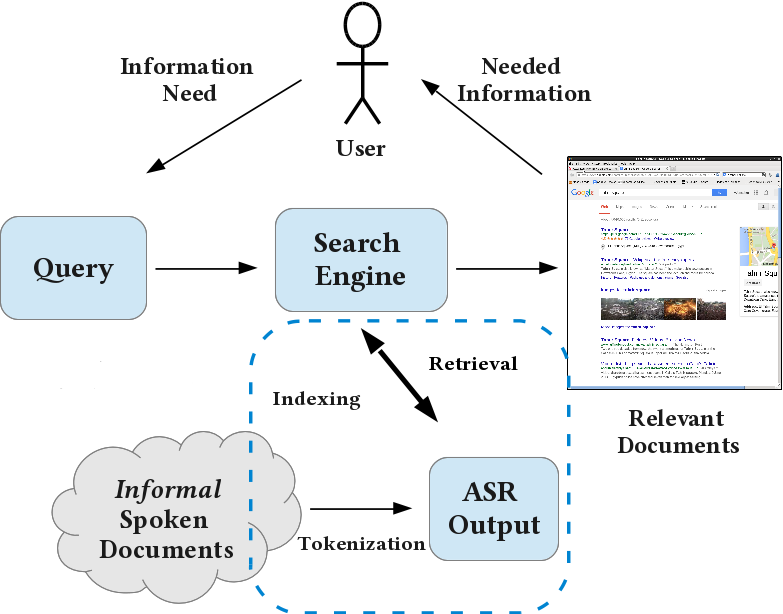
\includegraphics[width=0.7\textwidth]{sdr.png}
 \caption[Typical speech retrieval workflow]{A typical speech retrieval workflow. \label{fig:sdr}}
\end{figure}

However, when NIST revisited the issue in 2006 with the Spoken Term Detection evaluation\cite{std06eval}, a different set of conclusions emerged.  The 2006 evaluation focused on informal speech and languages other than English (Mandarin Chinese and Levantine Arabic) and on conversational speech in addition to the traditional broadcast news domain.  Performance on these other languages were about 50\% worse than the English systems.  Additionally, by treating ASR output as distinct from plain text, techniques such as indexing multiple ASR hypotheses led to significant gains over the black-box approach from the 2000 TREC eval.\cite{fiscus2007}  

For this reason Figure~\ref{fig:sdr} shows the tokenization, indexing, and retrieval steps in the overall workflow broken out explicitly.  We would consider the application of topic information to all three areas of the speech retrieval process.
 

 
\section{Topics in Recognition and Retrieval}

An additional aspect of 2006 NIST evaluation, the evaluation criteria, suggests that incorporating topic information is a reasonable direction to explore in with respect to extracting information from spoken content a language-rich digital environment.  Rather than evaluate speech recognition as a \textit{transcription} task, where accuracy is measured over all words in the corpus - i.e. the word error rate (WER), the 2006 and subsequent evaluations focused on the retrieval of key words and phrases.  In other words, we would measure our system accuracy not over all words, but the information-rich `topic' words.

If we look at model-based retrieval, which arises in the literature as text categorization or classification (e.g., spam filters, document routing, author attribution), we find that most algorithms operate on bags-of-words, which are simply \textit{accumulated token counts}.   As a consequence, we need not be constrained by the accuracy of particular token instances - the WER - and can attempt the task with \textit{limited training} higher WER systems.

For this reason we would like to focus on introducing topic information into the retrieval pipeline.   We focus on the term detection or keyword search task as our particular instantiation of speech retrieval in keeping with recent evaluations (cf. \cite{std06eval}, \cite{babel}).   For both the tokenization step and for indexing/retrieval we direct our emphasis at adding topic information to the modeling of word sequences: \textit{language modeling}.

For tokenization or ASR, the basic statistical question is to identify the most likely sequence of words given the observed acoustic signal.  Also described as the noisy channel model of ASR, we often see this expressed as:
\begin{equation}
\hat{W} = \argmax_{W} P(W|O) \approx \argmax_{W} P(O|W)\cdot P(W)
\end{equation}
We will make a reasonable simplifying assumption that the acoustics of a word, $P(O|W)$, are unrelated to any topic information about a particular word instance.  Which again brings our focus to the latter component of a type speech recognizer, the language model $P(W)$.

Similarly, for keyword retrieval, we are interested in the likelihood of the query word or phrase at a particular time instance, which we can also express by the above equation, only without the `$\argmax$'.  So for both recognition and retrieval we will discuss what topic information can be included in the \textit{\textbf{language model}}.

Typically, and particularly so for ASR, the language model for a word sequence $W$ of $m$ words, usually denoted as $w_1,\ldots,w_m$, is expressed, via the chain rule, as the product of the individual word probabilities conditioned on a short word history or word \textit{context}.
\begin{equation}
p(W) = \prod\limits_{i=1}^m{p(w_i|\Phi(w_i))}
\end{equation}
In all major commercial ASR systems this context is expressed assumed to be the $(N-1)$ words immediately preceding $w_i$, hence the N-gram language model.   However, we chose to let $\Phi(w_i)$ stand for any \textbf{\textit{context}} that influences the occurrence of $w_i$ - N-grams, syntax, repetitions, or \textbf{\textit{topic information}}.
%\section{Topic as Word Context}

The specific goal of this thesis then is to relate the two modes of topic information, subject-relatedness and locality, which we informally refer to as broad and local topic context, to formal language models.  Both broad and local contexts influence word usage in language and we show that by modeling word in such a manner improves speech recognition and retrieval tasks.  

% % % % % %  OK % % % % % % % % %

\section{Contributions}
\label{sec:contributions}
We aim to analyze the behavior of topic information in informal speech and to model that behavior in ways to improve speech retrieval applications.  

%We will demonstrate the robustness of the topic signal under errorful tokenization.   
\textbf{Locality for Topic Classification} - We will demonstrate that a temporal analysis of the topic signal (locality) can be used to improve topic classification of informal speech.

\textbf{Locality and Topicality for Speech Retrieval} - We will demonstrate that we can model both locality of word usage and subject relevance to improve speech retrieval.  We show locality can be expressed implicitly as part of the retrieval task, but also explicitly as part of the language model for the speech recognition component of the retrieval task.  

\textbf{Cauche-augmented Latent Topic Models} -  We will capture our intuition from the previous two results and describe a latent topic model that incorporates both the subject-relevance aspect of topicality as well as locality or repetition-based properties.  We demonstrate that broad and local context, as we have defined them, are complementary sources of information when applied to speech recognition and retrieval.  


\section{Outline}
\label{sec:outline}

The rest of this thesis is organized as follows.   In Chapter 2 we present background materiel placing the notion of `topic' in context with classification, language modeling, speech recognition and retrieval.  We aim to present a concise picture about how different techniques have been used to incorporate topic information into speech and language processing.   Chapter 3 examines how topics and location interact in classification-based retrieval of speech.  We also show how retrieval metrics provide a better gauge of system error with respect to topic-related tasks than tradition word-level transcription metrics.

In Chapter 4 we present three approaches relating to how topic information both in terms of locality and subject-relevance can be applied to language models and to speech retrieval.   We formalize this intuition in Chapter 5 and present a set of locality-aware latent topic models targeted for speech recognition and retrieval.   In Chapter 6 we analyze the ability of our proposed models to capture both aspects of topicality and in Chapter 7 we focus on our model's application to the speech retrieval task.  Finally, we summarize the individual components and their connection to topicality in speech and discuss possible directions for future work.
